\section{Introduction and Background}

\subsection{Climate Change and Heat-Health Impacts in the Johannesburg Context}

Climate change has driven a global temperature increase of over 1.2°C since the Industrial Revolution, with African regions experiencing higher-than-average temperature increases \citep{IPCC2024}. Urban areas are particularly affected due to development patterns and land use changes, with high temperatures increasingly linked to mortality and morbidity, especially during heatwaves \citep{Gasparrini2015, Analitis2018, Romanello2023}.

Heat-related risks are rising in Johannesburg at 1753 meters elevation with over 5.87 million inhabitants \citep{Worldometer2023}. The city recorded its highest temperature of 38°C in January 2016, breaking the previous record of 36.5°C from November 2015 \citep{Strydom2016}. Studies show that above a threshold of approximately 18.7°C apparent temperature, all-cause mortality rises by 0.9\% per 1°C increase and by 2.1\% per 1°C among seniors \citep{Wichmann2017, Scovronick2018}. While official records counted only 11 direct heat-related deaths in a recent assessment, researchers estimate the actual heat burden to be much higher \citep{Chersich2023}.

Climate models project substantial warming for Johannesburg. By late-century under a high-emissions scenario, mean annual temperatures in interior South Africa could rise 6--7°C above late 20th-century baselines \citep{Engelbrecht2015}. Even by 2050, Johannesburg may warm by approximately 2°C if global emissions remain high \citep{Engelbrecht2015, Souverijns2022}, with hot nights (minimum temperature >20°C) projected to quadruple from about 10 per year to approximately 40 per year -- and up to 100 in the city's most heat-prone neighbourhoods \citep{WorldBank2024}. Researchers estimate an additional 3--4 weeks of very hot days per year by mid-century \citep{Garland2015}, and the IPCC warns that beyond +2°C of global warming, heat-attributable mortality and morbidity in Africa will sharply rise \citep{IPCC2022}.

\subsection{Socio-Spatial Inequity and Heat Vulnerability}

Johannesburg's subtropical highland climate features hot summer days (October-April), often with afternoon thundershowers, and dry, sunny winter days with cold nights (May-September) \citep{Tyson2000}. However, the city's socio-spatial layout -- largely a legacy of apartheid-era planning -- significantly shapes heat vulnerability patterns today. Historically, policies created wealthy, low-density suburbs with ample green spaces alongside dense townships with minimal vegetation or services \citep{Giombini2022, Venter2020}. This has resulted in stark contrasts in urban heat exposure, with lush neighbourhoods enjoying cooler microclimates, while nearby townships can be approximately 6°C hotter than the surrounding countryside \citep{WorldBank2024, Habitat2023}.

Housing quality differences further exacerbate exposure: informal housing can become significantly hotter, with indoor temperatures up to 15°C higher than in modern housing during the day \citep{Naicker2017}. Apartheid geography has effectively embedded vulnerability into Johannesburg's landscape, clustering heat risk in marginalized communities \citep{Strauss2019}.

\subsection{Research Context and Positionality}
This research builds upon ongoing work at the HE²AT Center, which has established baseline heat vulnerability assessment frameworks for South African cities \citep{Jack}. As a researcher within this initiative, I bring expertise in data science and machine learning methods to extend these frameworks through advanced statistical techniques. My position at the intersection of public health and climate science informs a multidisciplinary approach that aims to translate complex data into actionable health interventions. This work specifically addresses gaps in the Heat Center's existing vulnerability assessments by developing dynamic predictive models that can account for temporal changes in vulnerability patterns across Johannesburg's diverse socioeconomic landscape.

\subsection{Conceptual Framework and Research Gaps}

This research employs a comprehensive framework for heat vulnerability encompassing three interconnected dimensions: exposure, sensitivity, and adaptive capacity \citep{IPCC2022}. Figure \ref{fig:conceptual_framework} illustrates these relationships and their determinants within Johannesburg's urban context.

\begin{figure}[h]
\centering
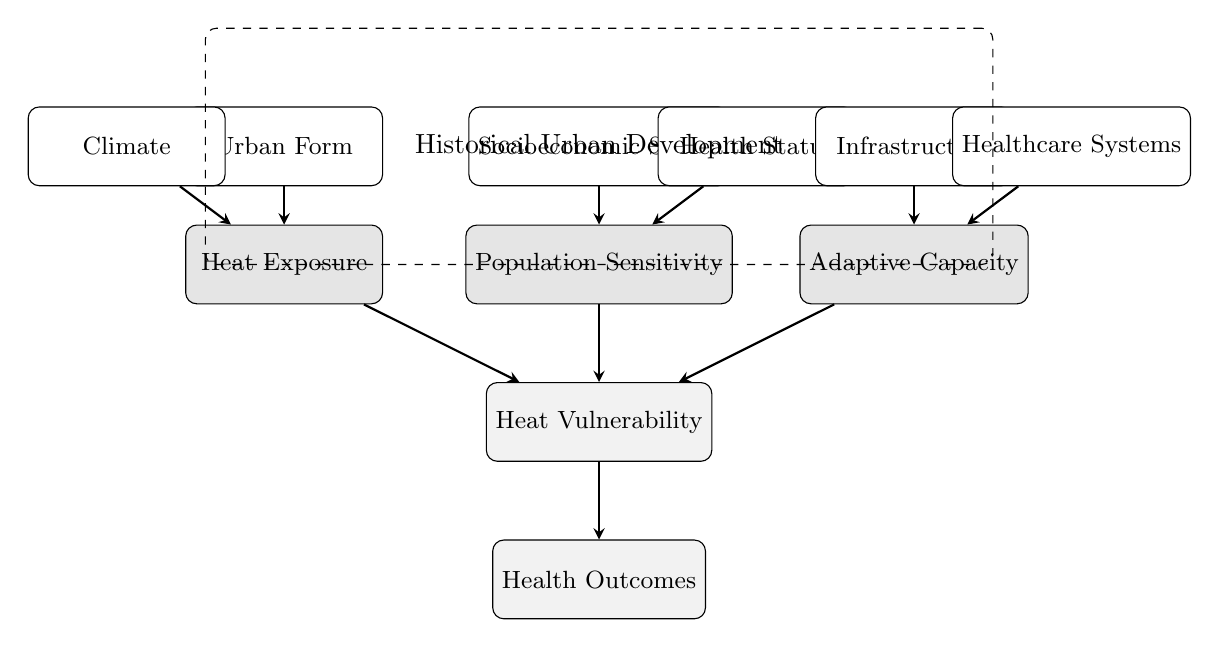
\begin{tikzpicture}[
    node distance=1.5cm,
    box/.style={rectangle, draw, rounded corners, minimum width=2.5cm, minimum height=1cm, text centered, font=\small},
    arrow/.style={thick, ->, >=stealth}
]

% Main components
\node[box, fill=gray!20] (exposure) at (0,0) {Heat Exposure};
\node[box, fill=gray!20] (sensitivity) at (4,0) {Population Sensitivity};
\node[box, fill=gray!20] (adaptive) at (8,0) {Adaptive Capacity};
\node[box, fill=gray!10] (vulnerability) at (4,-2) {Heat Vulnerability};
\node[box, fill=gray!10] (outcomes) at (4,-4) {Health Outcomes};

% Environmental factors
\node[box, fill=white] (urban) at (0,1.5) {Urban Form};
\node[box, fill=white] (climate) at (-2,1.5) {Climate};

% Socioeconomic factors
\node[box, fill=white] (socio) at (4,1.5) {Socioeconomic Status};
\node[box, fill=white] (health) at (6,1.5) {Health Status};

% Adaptation factors
\node[box, fill=white] (infra) at (8,1.5) {Infrastructure};
\node[box, fill=white] (systems) at (10,1.5) {Healthcare Systems};

% Connections
\draw[arrow] (exposure) -- (vulnerability);
\draw[arrow] (sensitivity) -- (vulnerability);
\draw[arrow] (adaptive) -- (vulnerability);
\draw[arrow] (vulnerability) -- (outcomes);

% Environmental connections
\draw[arrow] (climate) -- (exposure);
\draw[arrow] (urban) -- (exposure);

% Socioeconomic connections
\draw[arrow] (socio) -- (sensitivity);
\draw[arrow] (health) -- (sensitivity);

% Adaptation connections
\draw[arrow] (infra) -- (adaptive);
\draw[arrow] (systems) -- (adaptive);

% Historical influence
\node[draw, dashed, rounded corners, minimum width=10cm, minimum height=3cm] at (4,1.5) {Historical Urban Development};

\end{tikzpicture}
\caption{Conceptual framework of heat vulnerability in Johannesburg, highlighting the three primary dimensions (exposure, sensitivity, adaptive capacity) and their determinants. The dashed outline indicates components influenced by historical urban development patterns including apartheid-era planning.}
\label{fig:conceptual_framework}
\end{figure}

These components interact as follows:
\begin{itemize}
    \item \textit{Exposure} refers to heat stress degree and duration, with dense urban areas showing significantly higher surface temperatures (up to 5\textdegree C) compared to well-vegetated neighbourhoods \citep{Li2017, Santamouris2015}.
    
    \item \textit{Sensitivity} reflects population susceptibility influenced by socio-economic conditions and health status, with chronic conditions significantly increasing heat-related health risks \citep{Watts2023, Khosla2021, Souverijns2022}.
    
    \item \textit{Adaptive capacity} depends on access to healthcare, cooling infrastructure, and social support systems \citep{Ansah2024}, with limited access to healthcare affecting vulnerability to heat, as demonstrated by increased heat-related mortality in areas with restricted medical services \citep{Murage2020}.
\end{itemize}

\subsection{Recent Evidence on Heat Mortality}
Recent studies have strengthened our understanding of heat-mortality relationships in African urban contexts. Parker et al. \citep{Parker2023} demonstrated that in Johannesburg, heat vulnerability clusters in historically disadvantaged areas, with principal component analysis revealing environmental exposure explaining 31.5\% of variance, followed by health status (12.8\%) and socioeconomic conditions (12.3\%). Roffe et al. \citep{Roffe2023} projected intensification of heat stress conditions across southern Africa, with urban areas experiencing disproportionate impacts. The Lancet Countdown on Climate and Health \citep{Romanello2023} reports escalating impacts, with an estimated 5 million people globally dying annually from suboptimal temperatures, and approximately 37\% of heat-related mortality attributable to human-induced climate change \citep{Lancet2024}. The latest IPCC synthesis report \citep{IPCC2024} further emphasizes that climate-health impacts are accelerating fastest in resource-constrained urban environments, creating compounding vulnerabilities in African cities. These findings underscore the urgency of developing locally calibrated heat-health early warning systems for rapidly urbanizing African cities.

\subsection{Research Gaps in Urban African Contexts}
Despite growing climate health research worldwide, significant gaps remain in understanding the dynamics of heat health in urban African contexts. Most existing studies focus on high-income regions, overlooking the distinct characteristics of African cities \citep{Khine2023, Pasquini2020}. Key limitations include:

\begin{enumerate}
    \item \textbf{Scarcity of African Urban Heat-Health Studies:} Limited research examining the impacts of heat on health in African urban settings hinders the development of region-specific interventions \citep{Ncongwane2021, Wright2019}.

    \item \textbf{Siloed Disciplinary Approaches:} Lack of interdisciplinary collaboration results in fragmented insights that fail to capture the multifaceted nature of heat-health challenges \citep{Jack}.

    \item \textbf{Unique Urban Challenges:} African cities face distinct issues stemming from historical development patterns, unique disease profiles, and diverse urban morphologies requiring tailored research approaches \citep{Giombini2022, Venter2020}.
\end{enumerate}

Johannesburg exemplifies these challenges through its historical development and urban disparities \citep{Strauss2019}, high disease burden from both communicable and non-communicable diseases \citep{Wright2021}, and accelerated warming projections \citep{Engelbrecht2015, Souverijns2022}. Addressing these gaps is crucial for developing heat health strategies tailored to African urban contexts.